\documentclass{article}

% --- Packages ---
\usepackage[utf8]{inputenc} % Input encoding
\usepackage[T1]{fontenc}    % Font encoding
\usepackage{amsmath}        % Math formulas (though not heavily used here)
\usepackage{graphicx}       % Including images (if any) AND for \scalebox
\usepackage{listings}       % Code blocks
\usepackage[margin=1in]{geometry} % Set margins
\usepackage{hyperref}       % Clickable links (URLs, references)
\usepackage{abstract}       % For the abstract environment
\usepackage{color}          % Required for textcolor in listings postbreak hook
\usepackage{enumitem}       % For the enumerate environment
\usepackage{tikz}           % **** ADDED for flowchart ****
\usetikzlibrary{arrows.meta, shapes, positioning, calc} % **** ADDED for flowchart libraries ****
\usepackage{tabularx}

% --- 全局排版設置 ---
\sloppy             % 全局放寬排版要求,減少Overfull hbox
\hbadness=10000     % 提高underfull hbox警告閾值,減少不必要的警告

% --- Listing Configuration ---
% Basic configuration for code listings (adjust as needed)
\lstset{
  basicstyle=\ttfamily\small, % font type and size
  breaklines=true,            % automatically break long lines
  postbreak=\mbox{\textcolor{red}{$\hookrightarrow$}\space}, % symbol for broken lines
  language=bash               % default language
}

% --- Document Metadata ---
\title{A Unified Diagnostic Framework for GMAT Quantitative, Data Insights, and Verbal Sections}
\author{Yuchen Teng} %%%%<<< You might want to verify/change this
\date{\today}

% --- Document Start ---
\begin{document}

% 全域設置緩解排版問題
\sloppy
\hbadness=4000

\maketitle

\begin{abstract}
This paper presents a unified diagnostic framework for analyzing student performance in the quantitative (Q), data insights (DI), and verbal (V) sections of the GMAT. The framework employs a standardized chapter-based methodology to move beyond simple accuracy metrics, aiming to identify root causes of errors and inefficiencies. Core inputs include per-question data (time, correctness, type, difficulty, skill/domain), and overall test metrics. The analysis progresses through evaluating time strategy and data validity, conducting multidimensional performance analysis specific to each section\'s constructs, diagnosing error patterns (considering time, difficulty, and potential carelessness), applying coverage rules to detect widespread weaknesses, and generating personalized practice recommendations. The final output is a comprehensive diagnostic summary delivered in natural language, providing actionable insights and guidance for targeted student improvement. This unified structure ensures consistency in the analysis while accommodating the unique characteristics of each GMAT section.
\end{abstract}

\section{Introduction}

The Graduate Management Admission Test (GMAT) assesses critical reasoning, quantitative, data analysis, and verbal skills essential for graduate business programs. Effective preparation requires not only content mastery, but also strategic test-taking skills and an understanding of individual strengths and weaknesses. While numerous resources exist for practice, a systematic and standardized approach to diagnosing performance across all scored sections (Quantitative, Data Insights, Verbal) can significantly enhance study efficiency.

This paper introduces a unified diagnostic framework designed to provide in-depth analysis of student performance on the GMAT. Unlike simple score reports, this framework delves into the underlying reasons for errors and time inefficiencies, considering factors such as time pressure, question type, difficulty level, specific skills or content domains, and behavioral patterns.

The framework follows a consistent nine-chapter structure for analyzing each section (Q, DI, V), ensuring a comparable depth of insight while adapting the specific metrics and logic to the nuances of each section. This structure facilitates the following.

\begin{enumerate}
    \item \textbf{Standardized Input:} Defining core data requirements (Chapter 0).
    \item \textbf{Time \& Validity Assessment:} Evaluating Pacing and Filtering Unreliable Data (Chapter 1).
    \item \textbf{Multi-Dimensional Performance Analysis:} Examining performance across relevant section-specific dimensions (Chapter 2).
    \item \textbf{Root Cause Diagnosis:} Classifying errors and exploring the underlying causes (Chapter 3).
    \item \textbf{Section-Specific Analyses:} Investigating efficiency and patterns (Chapters 4 \& 5, adapted per section).
    \item \textbf{Coverage Assessment:} Identifying pervasive skill/type weaknesses (Chapter 6).
    \item \textbf{Personalized Recommendations:} Generating actionable practice plans (Chapter 7).
    \item \textbf{Synthesized Reporting:} Delivering a comprehensive, natural language summary (Chapter 8).
\end{enumerate}

% ***** FIGURE INSERTED HERE *****
\begin{figure}[htbp]
\centering
% Figure content first
\scalebox{0.78}{
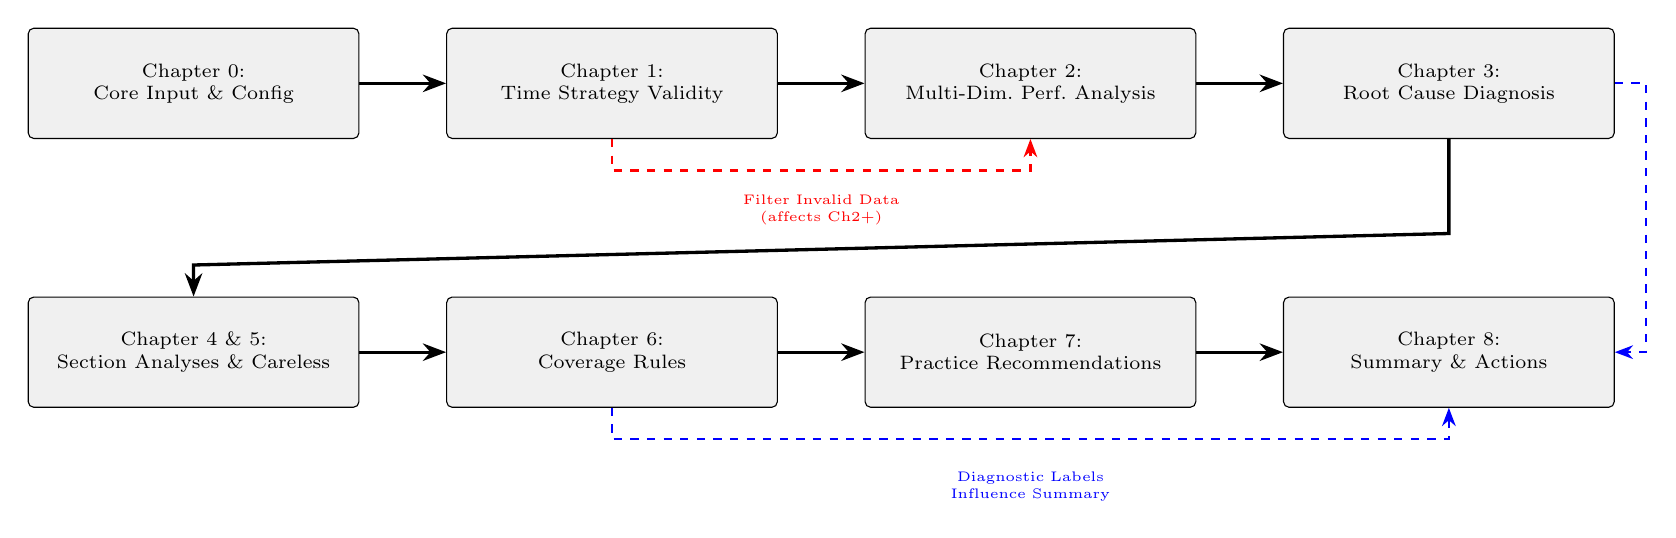
\begin{tikzpicture}[
  % --- styles ------------------------------------------------------------
  box/.style={
    rectangle, draw, rounded corners=2pt,
    minimum width=4.2cm, minimum height=1.4cm,
    font=\scriptsize, align=center, fill=gray!12
  },
  flow/.style={-Stealth, very thick},
  auxred/.style={-Stealth, dashed, red, thick},
  auxblue/.style={-Stealth, dashed, blue, thick},
  node distance = 2.0cm and 1.1cm
]

% --------------------- 1st row ------------------------------------------
\node[box] (ch0) {Chapter 0:\\Core Input \& Config};
\node[box, right=of ch0] (ch1) {Chapter 1:\\Time Strategy Validity};
\node[box, right=of ch1] (ch2) {Chapter 2:\\Multi‑Dim.\ Perf.\ Analysis};
\node[box, right=of ch2] (ch3) {Chapter 3:\\Root Cause Diagnosis};

% --------------------- 2nd row ------------------------------------------
\node[box, below=of ch0] (ch4) {Chapter 4 \& 5:\\Section Analyses \& Careless}; % Replaced U+202F with standard space
\node[box, right=of ch4] (ch6) {Chapter 6:\\Coverage Rules};
\node[box, right=of ch6] (ch7) {Chapter 7:\\Practice Recommendations};
\node[box, right=of ch7] (ch8) {Chapter 8:\\Summary \& Actions};

% --------------------- main flow arrows ---------------------------------
\draw[flow] (ch0) -- (ch1);
\draw[flow] (ch1) -- (ch2);
\draw[flow] (ch2) -- (ch3);

% ch3 ➜ ch4 (go down then left to avoid crossing the first row)
\coordinate (downR) at ($(ch3.south)+(0,-1.2)$);
\coordinate (downL) at ($(ch4.north)+(0,0.4)$);
\draw[flow] (ch3.south) -- (downR) -- (downL) -- (ch4.north);

\draw[flow] (ch4) -- (ch6);
\draw[flow] (ch6) -- (ch7);
\draw[flow] (ch7) -- (ch8);

% --------------------- red auxiliary arrow ------------------------------
%  ↓  vertical drop from ch1, then horizontal to ch3.south
\draw[auxred]
  ($(ch1.south)+(0,0)$) |- ($(ch1.south)+(0,-0.4)$) -| (ch2.south);

\node[font=\tiny, red, text width=2.7cm, align=center]
     at ($(ch1.south)!0.5!(ch2.south) + (0,-0.9)$)
     {Filter Invalid Data (affects Ch2+)};

% --------------------- blue diagnostic loop -----------------------------
\draw[auxblue] (ch3.east) -| ($(ch8.east)+(0.4,0)$) |- (ch8.east);
\draw[auxblue] (ch6.south) |- ($(ch8.south)+(0,-0.4)$) -| (ch8.south);

\node[font=\tiny, blue, text width=2.7cm, align=center]
     at ($(ch6.south)!0.5!(ch8.south) + (0,-1.0)$)
     {Diagnostic Labels\\Influence Summary};

\end{tikzpicture}} % End of \scalebox

% ***** VERTICAL SPACE ADDED HERE *****
\vspace{\baselineskip}

% Caption and label after the space
\caption{Overall Flow of the Unified Diagnostic Framework}
\label{fig:framework_flow}

\end{figure}
% ***** END OF FIGURE CODE *****


By applying this unified framework, students and instructors can gain a holistic understanding of performance, identify specific areas requiring intervention, and develop targeted strategies for improvement throughout the GMAT exam. The subsequent sections detail the methodology applied within each chapter of this framework.

\textit{Note on Document Purpose:} This document serves primarily as a technical report detailing the design, logic, and implementation rationale behind the unified GMAT diagnostic framework. It is intended as comprehensive documentation for users of the associated analysis tools (e.g., on GitHub) and as a methodological reference outlining the systematic approach developed. While initial parameters are informed by practical experience and preliminary testing, the core contribution presented here is the formalization of the diagnostic process itself.

Although experienced GMAT instructors often provide valuable information based on score reports, traditional analysis can suffer from subjectivity and inconsistency. Relying solely on intuition or anecdotal patterns introduces variability and hinders iterative refinement. Recognizing these limitations, the main motivation behind developing this unified diagnostic framework was to establish a more scientific, systematic, and objective approach. The goal is to enhance the efficiency, accuracy, and reliability of GMAT performance diagnosis by replacing purely experiential interpretation with a structured, parameterized, and verifiable methodology. The goal is to enhance the efficiency, accuracy, and reliability of GMAT performance diagnosis by replacing purely experiential interpretation with a structured, parameterized, and verifiable methodology.

\section{Methodology: The Diagnostic Framework}

\subsection{Framework Development Methodology} % Replacing existing content

The development of this unified diagnostic framework originated from the practical need to structure insights gained through analyzing student GMAT performance, combining quantitative score report data with qualitative follow-up. Initial quantitative analysis relied on custom logic applied to performance metrics, while qualitative assessment, such as comparing student approaches to specific problems, aimed to uncover cognitive obstacles not evident in the raw data.

To establish a replicable process, consultations were transcribed and analyzed, utilizing AI assistance to consolidate the underlying analytical logic and structure. A key phase involved the explicit formalization of the diagnostic workflow, transforming subjective or ambiguous rules (e.g., "significant time pressure") into precise, parameterized definitions and functions. The outputs of this logic were designed as computable diagnostic tags, facilitating the generation of recommendations or guiding further qualitative inquiry.

Validation proceeded iteratively by comparing the framework's automated analysis against independent expert evaluations on real data. Discrepancies informed refinements to the logic, parameters, and functions, ensuring closer alignment with established diagnostic practices. The core framework was subsequently implemented as an automated tool using Python, a process involving learning logical control flow, modular design, and debugging techniques.

Throughout development, considerations for end-users—both students seeking intuitive interaction and instructors requiring detailed, traceable diagnostics—influenced design choices, leading to concepts like AI-assisted interfaces and standardized output tagging. This process highlighted that while AI can assist, the core analytical logic must be soundly defined by the expert. It also emphasized the need for maintainable code structure when dealing with AI-generated or complex components.

This narrative provides context for the detailed methodology presented in the subsequent chapters.

% The original list-based methodology steps are removed and replaced by the text above.

% The next subsection starts here:
\subsection{Chapter 0: Core Input Data and Configuration}

\textbf{Objective:} Define the foundational data structures, parameters, and pre-processing steps required for analysis.

\textbf{Required Input CSV Structure:}
For the analysis scripts to function correctly, the input CSV file (e.g., \texttt{testset-q.csv}) must contain specific columns with data in the expected format. While column names can sometimes be adapted during implementation, the following represents the ideal structure and data types:

\begin{itemize}
    \item \texttt{question\_id}: Unique identifier for each question (String or Integer).
    \item \texttt{question\_time}: Response time for the question in minutes (Numeric, e.g., Float or Integer).
    \item \texttt{is\_correct}: Indicator of correctness (Boolean: \texttt{True}/\texttt{False}, or Integer: \texttt{1}/\texttt{0}).
    \item \texttt{question\_difficulty}: Numeric difficulty value (Numeric). The source might differ (e.g., \texttt{DI\_b}, \texttt{V\_b}), but it's mapped internally.
    \item \texttt{question\_position}: Sequence number of the question in the test (Integer, 1-indexed).
    \item \texttt{question\_type}: Category of the question (String). Specific values depend on the section:
        \begin{itemize}
            \item Q: 'Real' or 'Pure'.
            \item DI: 'DS', 'TPA', 'MSR', or 'GT'.
            \item V: 'CR' or 'RC'.
        \end{itemize}
    \item \texttt{question\_fundamental\_skill} (Required for Q and V): Core skill or domain tested (String, e.g., 'Rates/Ratio/Percent', 'Identify Stated Idea').
    \item \texttt{content\_domain} (Required for DI): Classification as 'Math Related' or 'Non-Math Related' (String).
\end{itemize}

\textbf{Overall Metrics (Derived or Input):}
While not always direct columns, the analysis requires:
\begin{itemize}
    \item \texttt{total\_test\_time} (Total minutes spent).
    \item \texttt{max\_allowed\_time} (Standard 45 minutes per section).
    \item \texttt{total\_number\_of\_questions}.
\end{itemize}

\textbf{Common Inputs:}
\begin{itemize}
    \item \textbf{Per-Question:} Requires fields such as \texttt{question\_id} (Identifier), \texttt{question\_time} (Response Time in minutes), \texttt{is\_correct} (Correctness as Boolean), \texttt{question\_difficulty} (Numeric value, potentially section-specific source like \texttt{DI\_b} or \texttt{V\_b}), \texttt{question\_position} (Sequence number).
    \item \textbf{Overall:} Requires \texttt{total\_test\_time} (Total minutes), \texttt{max\_allowed\_time} (standardized at 45 minutes per section), and \texttt{total\_number\_of\_questions}.
\end{itemize}

\textbf{Section-Specific Inputs \& Pre-processing:}
\begin{itemize}
    \item \textbf{Quant (Q):}
    \begin{itemize}
        \item Inputs: \texttt{question\_type} categorized as 'Real' (word problems) or 'Pure' (computation/concept); \texttt{question\_fundamental\_skill} representing core mathematical areas, e.g.:
            \begin{itemize}
                \item \texttt{Rates/Ratio/Percent}
                \item \texttt{Value/Order/Factor}
                \item \texttt{Equal/Unequal/ALG}
                \item \texttt{Counting/Sets/Series/Prob/Stats}
            \end{itemize}
        \item Pre-processing: Calculate \texttt{average\_time\_per\_type}, \texttt{max\_correct\_difficulty\_per\_skill}. Numerical conversions and handling of missing values are performed.
    \end{itemize}
    \item \textbf{Data Insights (DI):}
    \begin{itemize}
        \item Inputs: \texttt{question\_type} ('DS', 'TPA', 'MSR', 'GT'); \texttt{content\_domain} ('Math Related'/'Non-Math Related'). Note: \texttt{Fundamental Skills} are typically not tracked for DI.
        \item Pre-processing: Derive \texttt{average\_time\_per\_type}, \texttt{max\_correct\_difficulty\_per\_combination} (based on \texttt{question\_type} and \texttt{content\_domain}). A key step involves identifying \texttt{MSR} item sets (typically 3 questions) and estimating \texttt{msr\_reading\_time} based on the time differential between the first question and the average of the subsequent two: \texttt{reading\_time = time\_q1 - (time\_q2 + time\_q3) / 2}.
    \end{itemize}
    \item \textbf{Verbal (V):}
    \begin{itemize}
        \item Inputs: \texttt{question\_type} ('CR'/'RC'); \texttt{question\_fundamental\_skill}, e.g.:
            \begin{itemize}
                \item \texttt{Plan/Construct}
                \item \texttt{Identify Stated Idea}
                \item \texttt{Identify Inferred Idea}
                \item \texttt{Analysis/Critique}
            \end{itemize}
        \item Pre-processing: Identify \texttt{RC} passage groups (consecutive RC questions, usually 3-4). Calculate the following:
            \begin{itemize}
                \item \texttt{rc\_group\_id}
                \item \texttt{questions\_in\_group}
                \item \texttt{group\_total\_time}
                \item \texttt{average\_time\_per\_type}
                \item \texttt{first\_third\_average\_time\_per\_type}
            \end{itemize}
            Estimate \texttt{rc\_reading\_time} using a similar logic to MSR:
            \texttt{reading\_time = time\_q1 - average\_time\_of\_other\_qs\_in\_group}.
    \end{itemize}
\end{itemize}

\textbf{Implementation Context:} Data ingestion typically involves reading CSV files using libraries like \texttt{pandas}. Pre-processing includes data type conversion (e.g., \texttt{pd.to\_numeric}), handling missing data (\texttt{dropna}), mapping raw inputs (e.g., full question type names to abbreviations like 'CR'), renaming columns for consistency, and computing the derived metrics mentioned above. Configuration parameters (thresholds, factors) are defined constants within the implementation.

\textbf{Rationale:} Establishes a consistent, clean, and enriched data foundation crucial for reliable and comparable diagnostics across sections.

\subsection{Chapter 1: Overall Time Strategy and Data Validity Assessment}

\textbf{Objective:} Evaluate overall pacing, assess time pressure, establish section-appropriate overtime criteria, and identify potentially invalid data points resulting from rushed end-section performance.

\textbf{Operational Logic:}
\begin{enumerate}
    \item \textbf{Calculate Time Difference (\texttt{time\_diff}):} Computed as \texttt{max\_allowed\_time} - \texttt{total\_test\_time}.
    \item \textbf{Determine Time Pressure Status (\texttt{time\_pressure}):} This Boolean flag is determined by section-specific rules, generally combining \texttt{time\_diff} with evidence of rushed responses in the final third of the test.
    \begin{itemize}
        \item Q/DI: \texttt{time\_pressure} = \texttt{True} if \texttt{time\_diff} $\leq$ 3.0 minutes AND \texttt{question\_time} < 1.0 minute for any question in the last third.
        \item V: \texttt{time\_pressure} = \texttt{True} if \texttt{time\_diff} \leq 3.0 minutes AND \texttt{question\_time} < 1.0 minute for any question in the last third (aligning with Q/DI rule).
        \item A user override option (\texttt{user\_override\_time\_pressure}) allows manual setting of this flag.
    \end{itemize}
    \item \textbf{Establish Overtime Thresholds/Rules:} These criteria are dynamically set based on the \texttt{time\_pressure} status and vary by section and question type.
    \begin{itemize}
        \item \textbf{Q:} A single \texttt{overtime\_threshold} (e.g., 2.5 min if \texttt{time\_pressure}, 3.0 min otherwise).
        \item \textbf{DI:} Type-specific thresholds (e.g., \texttt{overtime\_threshold\_ds}: 2.0 min if \texttt{time\_pressure}, 2.5 otherwise; \texttt{overtime\_threshold\_tpa}: 3.0 min if \texttt{time\_pressure}, 3.5 otherwise; \texttt{overtime\_threshold\_gt}: 3.0 min if \texttt{time\_pressure}, 3.5 otherwise) and \texttt{MSR} group rules (\texttt{msr\_group\_target\_time}: 6.0 min if \texttt{time\_pressure}, 7.0 otherwise). Includes \texttt{MSR} single-question time analysis thresholds (\texttt{msr\_reading\_threshold}=1.5 min, \texttt{msr\_single\_q\_threshold}=1.5 min).
        \item \textbf{V:} Separate thresholds/rules for \texttt{CR} (\texttt{overtime\_threshold\_cr}: 2.0 min if \texttt{time\_pressure}, 2.5 otherwise) and \texttt{RC} (e.g., \texttt{rc\_group\_target\_time} for 3Q group: 6.0 min if \texttt{time\_pressure}, 7.0 otherwise; for 4Q group: 8.0 min if \texttt{time\_pressure}, 9.0 otherwise; \texttt{rc\_individual\_q\_threshold}=2.0 min). V also includes a preliminary check for \texttt{reading\_comprehension\_barrier\_inquiry} based on estimated \texttt{rc\_reading\_time} exceeding thresholds (e.g., >2.0 min for 3Q group, >2.5 min for 4Q group).
    \end{itemize}
    \item \textbf{Identify Invalid Data (\texttt{is\_invalid}):} This flag identifies questions likely answered without genuine effort due to time constraints. The logic is as follows:
        \begin{itemize}
            \item \textbf{Trigger Condition:} Only executed if \texttt{time\_pressure} == \texttt{True}.
            \item \textbf{Scope:} Only checks questions in the final third (\texttt{question\_position} > \texttt{Total Number of Questions} * 2/3).
            \item \textbf{Criteria Definition ("Abnormally Fast Response"):} A question (or its group for RC/MSR) is considered abnormally fast if it meets \textbf{at least one} of the following standards:
                \begin{itemize}
                    \item Absolute Time 1: \texttt{question\_time} < 0.5 minutes.
                    \item Absolute Time 2: \texttt{question\_time} < 1.0 minute.
                    \item Relative Single Question Time: \texttt{question\_time} < (Average time for that question type in the first third * 0.5).
                    \item Relative Group Time (RC/MSR only): \texttt{group\_total\_time} < (Average RC/MSR time in first third * Number of questions in group * 0.5).
                \end{itemize}
            \item \textbf{Flagging Logic:} If a question within the scope meets the trigger condition and satisfies \textit{any} of the "Abnormally Fast Response" criteria, it is flagged as \texttt{is\_invalid} = \texttt{True}.
        \end{itemize}
    \item \textbf{Global Rule - Data Filtering and Overtime Flagging:}
    \begin{itemize}
        \item First, apply the \texttt{is\_invalid} flag based on the logic above.
        \item Create a filtered dataset by removing questions marked \texttt{is\_invalid}. \textbf{All subsequent analyses (Chapters 2-7) exclusively use this filtered data.}
        \item Second, using the filtered dataset, apply the established overtime thresholds/rules to flag remaining questions with \texttt{overtime} = \texttt{True} (or section-specific variants like \texttt{group\_overtime} in V, \texttt{msr\_group\_overtime} in DI).
    \end{itemize}
\end{enumerate}

% ***** PASTE THE FIGURE CODE BLOCK HERE *****
    \begin{figure}[htbp]
    \centering
    % --- 使用 \scalebox 縮放圖表 ---
    \scalebox{0.51}{ % <-- 將tikzpicture包在裡面,0.9是縮放比例,您可以嘗試 0.85, 0.8 等等
    \begin{tikzpicture}[
        box/.style={rectangle, draw, rounded corners, minimum width=3cm, minimum height=0.8cm, text centered, font=\small, align=center},
        decision/.style={diamond, draw, aspect=2, minimum width=4cm, minimum height=1.5cm, text centered, font=\small, align=center},
        arrow/.style={->, >=stealth, thick},
        param/.style={rectangle, draw, dashed, rounded corners, fill=yellow!20, font=\tiny, align=left, inner sep=2pt}, % Use tiny for params
        % Adjust node distance for wrap-around layout
        node distance=1.5cm and 1.0cm % Increased vertical, adjusted horizontal
    ]
    % Nodes - Row 1 (Left to Right)
    \node[box, fill=gray!10] (time_diff) {time\_diff = max\_allowed\_time \\ - total\_test\_time};

    \node[decision, right=of time_diff] (pressure_cond) {time\_diff $\leq$ 3.0min &\\Time for last 1/3 Q < 1.0min?};

    \node[box, right=of pressure_cond] (pressure_result) {time\_pressure = True};

    \node[decision, right=of pressure_result] (invalid_check) {Abnormally Fast Response\\in last 1/3?}; % <-- MODIFIED NODE TEXT

    % Nodes - Row 2 (Right to Left)
    \node[box, below=of invalid_check] (invalid_result) {is\_invalid = True};

    \node[box, fill=red!10, left=of invalid_result] (filter) {Filter questions\\marked as is\_invalid};

    \node[box, left=of filter] (overtime) {Calculate overtime thresholds\\based on filtered data};

    % Parameter Nodes (Positioned below main nodes)
    \node[param, below=of pressure_cond, yshift=0.5cm] (pressure_param) {Time Pressure Threshold: 3.0min\\Last 1/3 Q Threshold: 1.0min};

    \node[param, below=of invalid_check, yshift=0.5cm, text width=5.5cm] (invalid_param) {Trigger: time\_pressure=True & Pos > Tot*2/3.\\Criteria (OR): Q time < 0.5min; < 1.0min;\\< 50% avg 1st 1/3 (single);\\< 50% avg 1st 1/3 * N (RC/MSR group)}; % <-- MODIFIED PARAM TEXT

    \node[param, below=of overtime, yshift=0.5cm, text width=4.5cm] (overtime_params) {
        With Time Pressure / Without Pressure:\\
        Q: 2.5min / 3.0min\\
        DI-DS: 2.0min / 2.5min\\
        DI-TPA: 3.0min / 3.5min\\
        DI-GT: 3.0min / 3.5min\\ % <-- MODIFIED THRESHOLD
        DI-MSR: 6.0min / 7.0min (Group)\\
        MSR Reading: 1.5min (Threshold)\\
        MSR Single Q: 1.5min (Threshold)\\\n        V-CR: 2.0min / 2.5min\\
        V-RC 3Q: 6.0min / 7.0min (Group)\\
        V-RC 4Q: 8.0min / 9.0min (Group)\\
        RC Individual: 2.0min (Threshold)
    };

    % Connections - Wrap-around flow
    \draw[arrow] (time_diff) -- (pressure_cond);
    \draw[arrow] (pressure_cond) -- node[above, font=\scriptsize, pos=0.4] {Yes} (pressure_result);
    \draw[arrow] (pressure_result) -- (invalid_check);
    \draw[arrow] (invalid_check) -- node[right, font=\scriptsize, pos=0.6] {Yes} (invalid_result); % Down arrow
    \draw[arrow] (invalid_result) -- (filter); % Left arrow
    \draw[arrow] (filter) -- (overtime); % Left arrow

    % Parameter Connections
    \draw[arrow, dashed] (pressure_param) -- (pressure_cond);
    \draw[arrow, dashed] (invalid_param) -- (invalid_check);
    \draw[arrow, dashed] (overtime_params) -- (overtime);

    \end{tikzpicture}
    } % <-- \scalebox 的結束括號
    % --- 結束 \scalebox ---
    
    \vspace{\baselineskip} % 如果您想保留圖表和標題間的距離
    \caption{Flowchart for Chapter 1 Logic: Time Pressure, Data Validity, and Overtime Thresholds}
    \label{fig:chapter1_logic}
    \end{figure}
    % ***** END OF FIGURE CODE *****

\textbf{Implementation Context:} Boolean flags (\texttt{time\_pressure}, \texttt{is\_invalid}, \texttt{overtime}) are added as columns to the \texttt{pandas} DataFrame. Thresholds are assigned to variables based on conditional logic applied to the \texttt{time\_pressure} status. Filtering is achieved via DataFrame slicing (e.g., \texttt{df\_filtered = df[\textasciitilde df['is\_invalid']]}).

\textbf{Rationale:} Ensures analyses are based on reliable data reflecting genuine effort and capability, while setting context-aware standards for time efficiency. Explicitly filtering invalid data before overtime flagging prevents misinterpreting rushed guesses as slow performance.

\subsection{Chapter 2: Multi-Dimensional Performance Analysis}

\textbf{Objective:} Analyze performance accuracy and efficiency across key dimensions relevant to each section, using the \textbf{filtered dataset}.

\textbf{Operational Logic:}
\begin{itemize}
    \item \textbf{Difficulty Level Standardization:} Raw numeric \texttt{question\_difficulty} values are mapped to standardized categorical bands (e.g., "Low / 505+", "Medium / 605+", "High / 705+") using a consistent mapping function across sections. This facilitates comparison and interpretation.
    \item \textbf{Performance Metric Calculation:} For each relevant dimension or combination, calculate key metrics using the filtered data: total count, number of errors (\texttt{is\_correct}==\texttt{False}), number of overtime instances (\texttt{overtime}==\texttt{True}), error rate, and overtime rate. Division by zero is handled gracefully (e.g., returning 0.0 or NaN).
\end{itemize}

\newpage
\textbf{Section-Specific Analysis Dimensions \& Metrics:}
\begin{itemize}
    \item \textbf{Quant (Q):}
    \begin{itemize}
        \item The primary dimensions analyzed for Quant section are: \texttt{question\_type} ('Real'/'Pure'), \texttt{question\_fundamental\_skill}, and \texttt{difficulty\_label}.
        \item Analysis: Compares error rates and overtime rates between 'Real' and 'Pure'. Identifies significant differences based on absolute count difference ($\geq$ 2) in errors or overtime instances, setting flags (\texttt{poor\_real}, \texttt{slow\_pure}, etc.).
    \end{itemize}
    \item \textbf{Data Insights (DI):}
    \begin{itemize}
        \item Dimensions: \texttt{content\_domain} ('Math Related'/'Non-Math Related'), \texttt{question\_type} ('DS', 'TPA', 'MSR', 'GT'), \texttt{difficulty\_label}.
        \item Analysis: Calculates error and overtime rates per dimension/combination. Identifies significant differences between \texttt{content\_domain}s based on absolute count difference ($\geq$ 2), setting flags (\texttt{poor\_math\_related}, \texttt{slow\_non\_math\_related}, etc.).
    \end{itemize}
    \item \textbf{Verbal (V):}
    \begin{itemize}
        \item Dimensions: \texttt{question\_fundamental\_skill}, \texttt{difficulty\_label}, \texttt{question\_type} ('CR'/'RC').
        \item Analysis: Calculates error rates per dimension/combination. Identifies difficulty ranges and skills with the highest error concentration.
    \end{itemize}
\end{itemize}

\textbf{Implementation Context:} \texttt{pandas} \texttt{groupby()} operations combined with \texttt{agg()} or \texttt{size().unstack()} are used extensively to compute metrics across dimensions. Error and overtime rates are calculated element-wise, often requiring intermediate steps to handle potential zero denominators (e.g., replacing 0 with \texttt{np.nan} before division). Significance flags are set using conditional logic based on the calculated metric differences.

\textbf{Rationale:} Pinpoint specific areas (types, skills, domains, difficulties) where accuracy or efficiency challenges exist within the valid performance data, providing focus for root cause diagnosis and practice planning.

\subsection{Chapter 3: Root Cause Diagnosis and Analysis}

\textbf{Objective:} Investigate the underlying reasons (\"why") for errors and inefficiencies identified in previous chapters, utilizing the \textbf{filtered dataset}.

\textbf{Core Concepts \& Operational Framework:}
\begin{enumerate}
    \item \textbf{Time Performance Classification:} Categorizes each valid question\'s time relative to the average for its type. Required metrics (\texttt{average\_time\_per\_type}) are pre-calculated from the filtered data.
    \begin{itemize}
        \item \texttt{is\_relatively\_fast}: \texttt{question\_time} < (\texttt{average\_time\_per\_type} * 0.75). The 0.75 factor is a configurable parameter.
        \item \texttt{is\_slow}: Determined by the \texttt{overtime} flag (or its variants) applied in Chapter 1 based on the filtered data.
        \item \texttt{is\_normal\_time}: Default state if neither \texttt{is\_relatively\_fast} nor \texttt{is\_slow}.
    \end{itemize}
    \item \textbf{Special Focus Error (\texttt{special\_focus\_error}, SFE):} This critical flag identifies instability in foundational knowledge.
    \begin{itemize}
        \item Definition: An error is classified as SFE under the following condition:
        \texttt{is\_correct} == False AND \texttt{question\_difficulty} < \texttt{max\_mastered\_difficulty}.
        \item \texttt{max\_mastered\_difficulty} is calculated per \texttt{question\_fundamental\_skill} (for Q/V) or per \texttt{question\_type}/\texttt{content\_domain} combination (for DI section) by finding the maximum \texttt{question\_difficulty} among correctly answered questions within that category in the filtered data.
        \item Handling: SFE-flagged questions receive priority in subsequent reporting and recommendation generation.
    \end{itemize}
    \item \textbf{Diagnostic Label Assignment:} Based on the time performance classification and SFE status, each question is assigned diagnostic labels. These labels encapsulate the primary findings regarding potential root causes (e.g., \"Slow \& Wrong\", \"Fast \& Wrong\", \"SFE\"). These labels, rather than complex scenarios, serve as the core input for generating targeted recommendations in Chapter 7 and the narrative summary in Chapter 8. The detailed follow-up actions (student recall, evidence review, qualitative analysis) are presented as guidance in Chapter 8.
\end{enumerate}

% ***** 在此處插入 Chapter 3 邏輯的圖表 *****
\begin{figure}[htbp]
\centering
% --- 這張圖很可能因為寬度需要縮放 ---
\scalebox{0.6}{ % <-- 建議從 0.8 開始嘗試縮放,如果仍太大,試試 0.75 或更小的數值
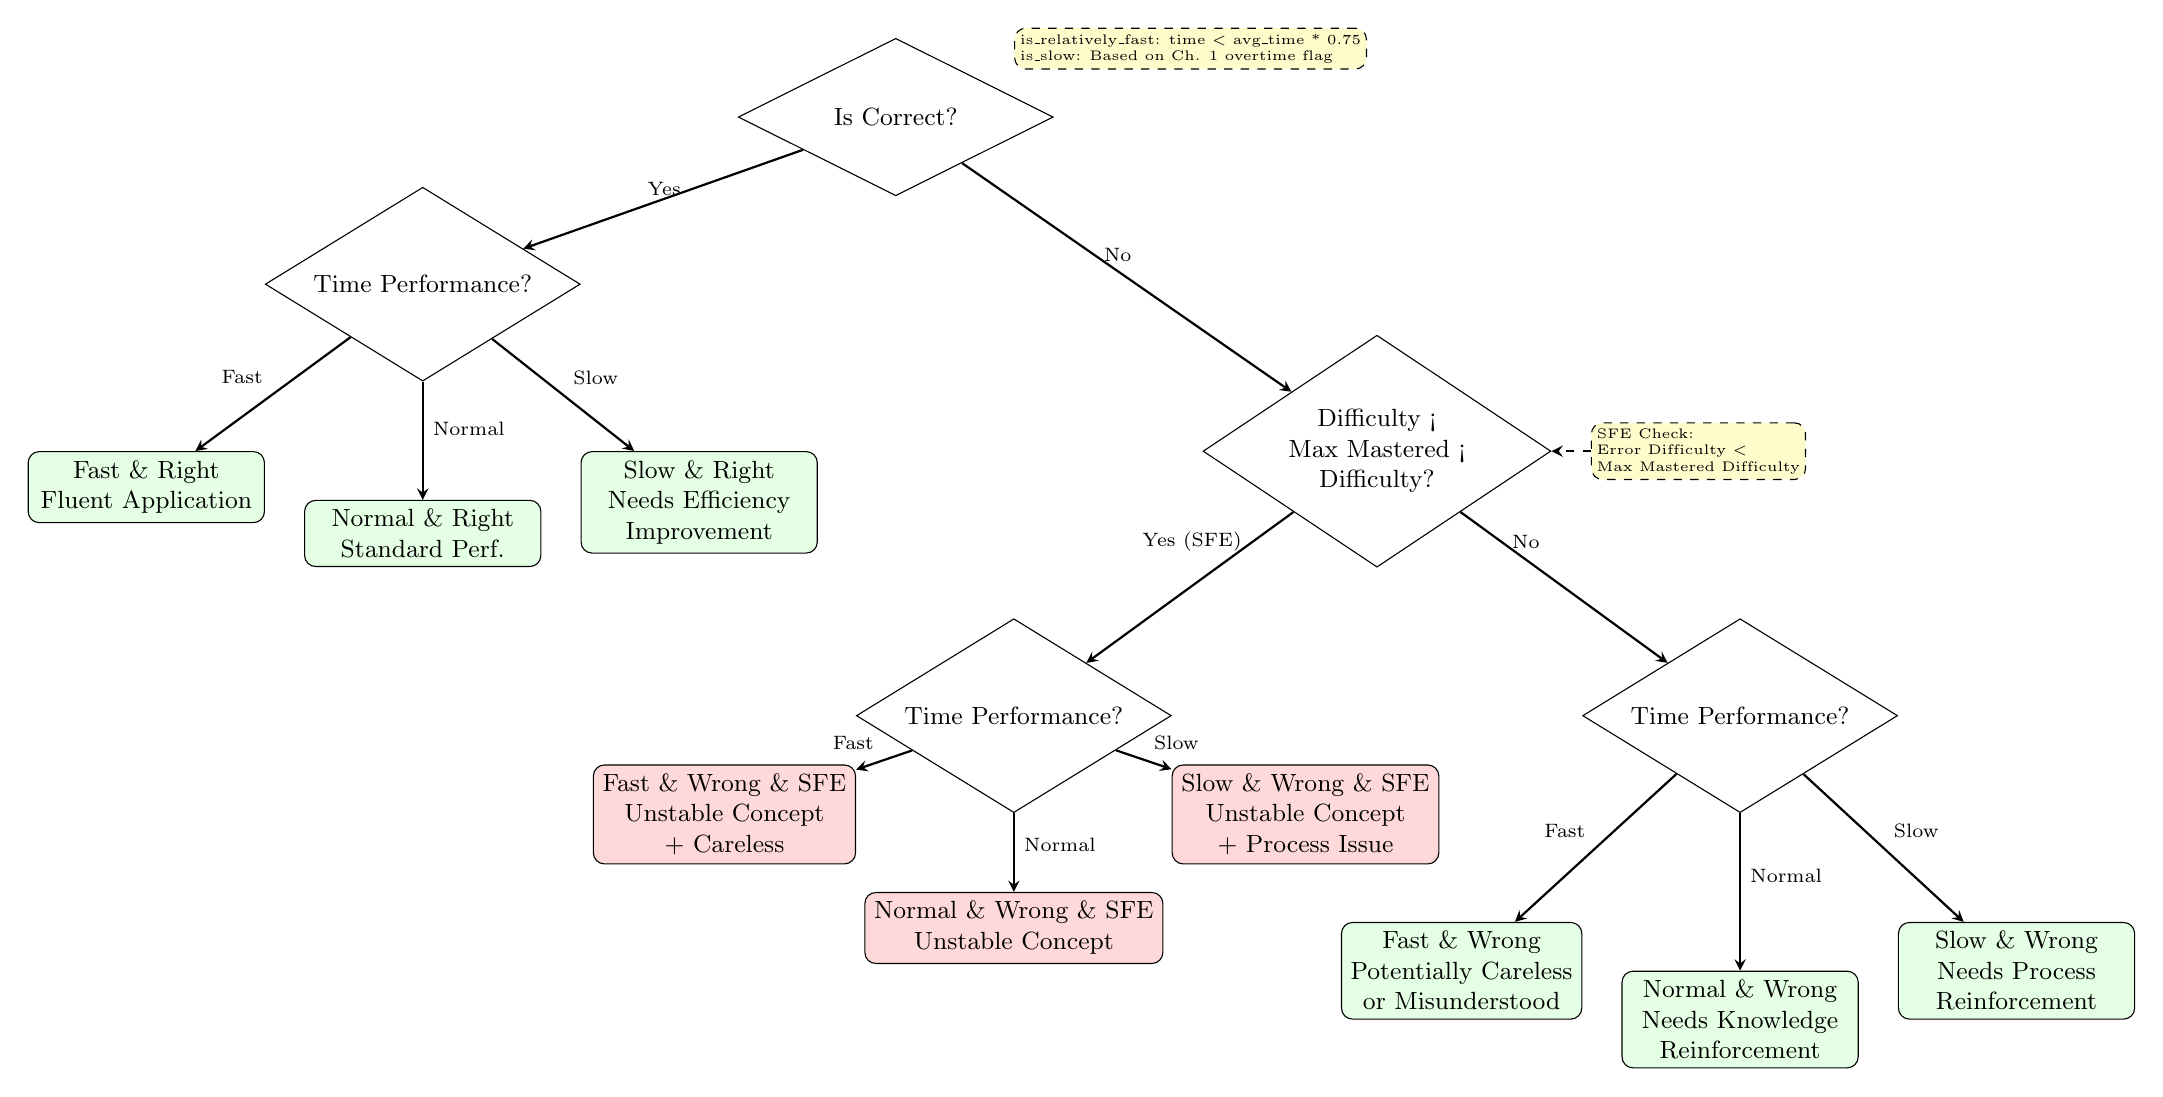
\begin{tikzpicture}[
    % General node distance (vertical and horizontal) - Increased vertical slightly
    node distance=2.5cm and 3cm, % Increased vertical base distance
    % Styles
    box/.style={rectangle, draw, rounded corners, minimum width=10cm, minimum height=10cm, text centered, font=\small, align=center}, % Adjusted min width/height - likely not needed if scaled
    decision/.style={diamond, draw, aspect=1.5, minimum width=4cm, minimum height=2cm, text centered, font=\small, align=center},
    leaf/.style={rectangle, draw, rounded corners, fill=green!10, minimum width=3cm, minimum height=0.8cm, text centered, font=\small, align=center},
    arrow/.style={->, >=stealth, thick},
    param/.style={rectangle, draw, dashed, rounded corners, fill=yellow!20, font=\tiny, align=left, inner sep=2pt}
]
% --- Root Node and Parameters ---
\node[decision] (is_correct) {Is Correct?};

\node[param, above right = 0.1cm and 0.5cm of is_correct] (time_params) {is\_relatively\_fast: time < avg\_time * 0.75\\is\_slow: Based on Ch. 1 overtime flag};

% --- Correct Branch (Seems OK, minor vertical adjust) ---
\node[decision, below left = 1cm and 4cm of is_correct] (correct_time) {Time Performance?}; % Increased horizontal dist slightly
\draw[arrow] (is_correct) -- node[left, pos=0.4, font=\scriptsize] {Yes} (correct_time);

\node[leaf, below left = 1.5cm and 1cm of correct_time] (fast_right) {Fast \& Right\\Fluent Application};
\node[leaf, below = 1.5cm of correct_time] (normal_right) {Normal \& Right\\Standard Perf.};
\node[leaf, below right = 1.5cm and 1cm of correct_time] (slow_right) {Slow \& Right\\Needs Efficiency\\Improvement};

\draw[arrow] (correct_time) -- node[above left, font=\scriptsize] {Fast} (fast_right);
\draw[arrow] (correct_time) -- node[right, pos=0.4, font=\scriptsize] {Normal} (normal_right);
\draw[arrow] (correct_time) -- node[above right, font=\scriptsize] {Slow} (slow_right);

% --- Incorrect Branch ---
% Position 'wrong_first' further right
\node[decision, below right = 3cm and 4cm of is_correct] (wrong_first) {Difficulty <\\Max Mastered <\\Difficulty?}; % Increased horizontal dist slightly
\draw[arrow] (is_correct) -- node[right, pos=0.4, font=\scriptsize] {No} (wrong_first);

\node[param, right = 0.5cm of wrong_first] (sfe_param) {SFE Check:\\Error Difficulty < \\Max Mastered Difficulty};
\draw[arrow, dashed] (sfe_param) -- (wrong_first);

% Increase horizontal separation for sub-branches drastically!
\node[decision, below left = 2cm and 2.5cm of wrong_first] (sfe_time) {Time Performance?}; % Was 1.5cm, now 4.5cm horizontal offset
\node[decision, below right = 2cm and 2.5cm of wrong_first] (normal_wrong_time) {Time Performance?}; % Was 1.5cm, now 4.5cm horizontal offset

\draw[arrow] (wrong_first) -- node[left, pos=0.2, font=\scriptsize] {Yes (SFE)} (sfe_time);
\draw[arrow] (wrong_first) -- node[right, pos=0.2, font=\scriptsize] {No} (normal_wrong_time);

% --- SFE Sub-branch Leaves (Adjust horizontal positioning relative to parent) ---
\node[leaf, below left = 0cm and 1cm of sfe_time, fill=red!15] (fast_wrong_sfe) {Fast \& Wrong \& SFE\\Unstable Concept\\+ Careless}; % Reduced internal horizontal spread
\node[leaf, below = 1cm of sfe_time, fill=red!15] (normal_wrong_sfe) {Normal \& Wrong \& SFE\\Unstable Concept}; % Increased vertical distance
\node[leaf, below right = 0cm and 1cm of sfe_time, fill=red!15] (slow_wrong_sfe) {Slow \& Wrong \& SFE\\Unstable Concept\\+ Process Issue}; % Reduced internal horizontal spread

\draw[arrow] (sfe_time) -- node[above left, font=\scriptsize] {Fast} (fast_wrong_sfe);
\draw[arrow] (sfe_time) -- node[right, pos=0.4, font=\scriptsize] {Normal} (normal_wrong_sfe);
\draw[arrow] (sfe_time) -- node[above right, font=\scriptsize] {Slow} (slow_wrong_sfe);

% --- Normal Wrong Sub-branch Leaves (Adjust horizontal positioning relative to parent) ---
\node[leaf, below left = 2cm and 1cm of normal_wrong_time] (fast_wrong) {Fast \& Wrong\\Potentially Careless\\or Misunderstood}; % Reduced internal horizontal spread
\node[leaf, below = 2cm of normal_wrong_time] (normal_wrong) {Normal \& Wrong\\Needs Knowledge\\Reinforcement}; % Increased vertical distance
\node[leaf, below right = 2cm and 1cm of normal_wrong_time] (slow_wrong) {Slow \& Wrong\\Needs Process\\Reinforcement}; % Reduced internal horizontal spread

\draw[arrow] (normal_wrong_time) -- node[above left, font=\scriptsize] {Fast} (fast_wrong);
\draw[arrow] (normal_wrong_time) -- node[right, pos=0.4, font=\scriptsize] {Normal} (normal_wrong);
\draw[arrow] (normal_wrong_time) -- node[above right, font=\scriptsize] {Slow} (slow_wrong);

\end{tikzpicture}
} % <-- \scalebox 的結束括號
\vspace{\baselineskip} % 您可以保留這個,在圖表和標題間增加垂直距離
\caption{Flowchart for Chapter 3 Logic: Root Cause Diagnosis Labels}
\label{fig:chapter3_logic}
\end{figure}
% ***** 圖表程式碼結束 *****

\textbf{Implementation Context:} The logic is implemented within the main analysis loop iterating through the filtered DataFrame. Time classification and SFE flags (serving as primary diagnostic labels) are computed for each question. These labels are stored, often alongside brief descriptive notes derived from the combination (e.g., potential cause hypotheses like \"calculation barrier\" for DI Math Slow \& Wrong), for use in generating detailed diagnostic text and recommendations in Chapters 7 and 8.

\textbf{Rationale:} Moves beyond identifying \textit{what} is wrong to systematically classifying \textit{why} using standardized diagnostic labels, enabling the development of targeted and effective improvement strategies by providing structured inputs for subsequent planning and reporting.

\subsection{Chapters 4 \& 5: Section-Specific Analyses, Patterns, and Carelessness}

\textbf{Objective:} Conduct further analyses tailored to section characteristics, examine efficiency in correct answers, and assess behavioral patterns like carelessness, using the \textbf{filtered dataset}.

\textbf{Synthesized Analyses \& Operationalization:}
\begin{itemize}
    \item \textbf{Analysis of Correct but Overtime Questions:}
    \begin{itemize}
        \item Identification: Filter questions where \texttt{is\_correct} == True AND \texttt{is\_slow} (or equivalent overtime flag) == True.
        \item Data Recorded: \texttt{question\_id}, \texttt{question\_type}, \texttt{question\_fundamental\_skill} (if applicable), \texttt{question\_time}.
        \item Purpose: These instances trigger recommendations in Chapter 7 aimed at improving fluency and efficiency.
    \end{itemize}
    \item \textbf{Special Pattern Observation (Early-Stage Rapid Responses):}
    \begin{itemize}
        \item Identification: We check for questions meeting these criteria:
        Located in the first third (\texttt{question\_position} $\leq$ \texttt{total\_number\_of\_questions} / 3) AND \texttt{question\_time} < 1.0 minute (absolute threshold).
        \item Reporting: If found, an alert regarding potential pacing issues or \texttt{flag for review} risks is included in the Chapter 8 summary.
    \end{itemize}
    \item \textbf{Carelessness Assessment (\texttt{carelessness\_issue}):}
    \begin{itemize}
        \item Calculation: Determine \texttt{fast\_wrong\_rate} = (Count of \texttt{is\_relatively\_fast} AND \texttt{is\_correct} == False) / (Total count of \texttt{is\_relatively\_fast}). Requires prior calculation of the \texttt{is\_relatively\_fast} flag from Chapter 3. Handle division by zero if no questions were relatively fast.
        \item Flagging: If \texttt{fast\_wrong\_rate} > 0.25 (configurable threshold), set \texttt{carelessness\_issue} = \texttt{True}.
        \item Reporting: If flagged, the Chapter 8 summary includes a note about potential carelessness.
    \end{itemize}
    \item \textbf{DI-Specific Pattern Observation:} For the Data Insights section, specific patterns like Multi-Source Reasoning (MSR) time distribution (e.g., comparing reading time vs. question-solving time) are also examined to identify potential inefficiencies within complex item types.
    \item \textbf{Core Skill/Type Reference (Context for Verbal):} The detailed breakdown of \texttt{CR} and \texttt{RC} sub-types, originally presented as a separate chapter in the Verbal source document, serves as reference material for interpreting Chapter 3 diagnoses and formulating Chapter 7 recommendations for the Verbal section. It is not an active analytical step itself but provides necessary classification context.
\end{itemize}

\textbf{Implementation Context:} These analyses are typically performed after the main Chapter 3 loop. Identification involves conditional filtering of the DataFrame. Rate calculations use simple aggregation and division. Flags are stored for use in Chapter 8 report generation.

\textbf{Rationale:} These chapters refine the diagnosis by examining efficiency patterns even in correct responses, identifying potential test-taking habits (pacing, carelessness), and providing necessary contextual classification (for Verbal), thereby adding further layers to the performance understanding.

\subsection{Chapter 6: Fundamental Ability / Skill / Type Coverage Rules}

\textbf{Objective:} Determine if pervasive weakness exists across an entire \texttt{fundamental\_skill} (Q/V) or \texttt{question\_type} (DI), warranting foundational reinforcement rather than solely addressing individual errors, using the \textbf{filtered dataset}.

\textbf{Operational Logic:}
\begin{enumerate}
    \item \textbf{Calculate Performance Rates:} For each \texttt{fundamental\_skill} (Q/V) or \texttt{question\_type} (DI), compute the overall \texttt{error\_rate} and \texttt{overtime\_rate} using the filtered data.
    \item \textbf{Trigger Override:} A coverage rule is triggered if, for a given skill/type, \texttt{error\_rate} > 0.5 \textbf{OR} \texttt{overtime\_rate} > 0.5. The 0.5 (50\%) threshold is a configurable parameter. Set \texttt{skill\_override\_triggered}[\textit{Skill}] (Q/V) or \texttt{override\_triggered}[\textit{Type}] (DI) = \texttt{True}.
    \item \textbf{Determine Macroscopic Parameters (If Triggered):} These parameters guide the foundational practice recommendations.
    \begin{itemize}
        \item \textbf{Macroscopic Difficulty (\texttt{Y\_agg}):} Identify the minimum \texttt{question\_difficulty} among all error or overtime questions within the triggered skill/type. Map this minimum difficulty to the standardized 6-level label (e.g., "Low / 505+", "Medium / 605+").
        \item \textbf{Macroscopic Time Limit (\texttt{Z\_agg}):}
        \begin{itemize}
            \item Q: Fixed at 2.5 minutes.
            \item DI: Based on the maximum \texttt{question\_time} observed within the triggered type, rounded down to the nearest 0.5 minutes (\texttt{floor(max\_time\_triggering * 2) / 2}).
            \item V: Standard target times for the respective skill/type are used (e.g., CR 2.0 min, RC 1.5 min).
        \end{itemize}
    \end{itemize}
\end{enumerate}

\textbf{Implementation Context:} Performance rates are calculated using \texttt{groupby()} on the filtered DataFrame. The override trigger logic involves conditional checks on these rates. If triggered, \texttt{Y\_agg} is determined by finding the minimum difficulty in the relevant subset and applying the standard mapping function; \texttt{Z\_agg} is calculated based on the rules above. Results are typically stored in dictionaries mapping skills/types to their override status and associated \texttt{Y\_agg}/\texttt{Z\_agg} values.

\textbf{Rationale:} Acts as a crucial gating mechanism for practice planning. If a fundamental area shows systemic weakness (high error/overtime rate), the framework prioritizes broad, foundational practice (macroscopic recommendation) over potentially numerous, less effective fixes for individual symptoms (microscopic recommendations).

\subsection{Chapter 7: Practice Planning and Recommendations}

\textbf{Objective:} Translate all diagnostic findings from the filtered data analysis into a specific, actionable, and personalized practice plan.

\textbf{Operational Logic:}
\begin{enumerate}
    \item \textbf{Identify Recommendation Triggers:} Collate all instances requiring recommendations:
    \begin{itemize}
        \item Individual questions flagged as incorrect (\texttt{is\_correct}==False) or correct but overtime (\texttt{is\_correct}==True AND \texttt{is\_slow}==True) based on Chapters 3 \& 4 analyses.
        \item Skills (Q/V) or Types (DI) flagged by the override rule (\texttt{skill\_override\_triggered} / \texttt{override\_triggered}) in Chapter 6.
    \end{itemize}
    \item \textbf{Generate Recommendations (Iterative Process):}
    \begin{itemize}
        \item \textbf{Exemption Check:} Before generating a case-specific recommendation for a skill (Q/V) or type/domain combination (DI), check if it exhibits stable performance. This is determined by verifying if **all** valid questions within that category are **both correct AND not overtime**. If this condition is met (100% accuracy and 100% efficiency within valid data), the category is considered exempt, and case-specific recommendations for it are skipped. Exemption notes are recorded.
        \item \textbf{Override Check:} If a skill/type has its override flag set (\texttt{True} from Chapter 6), generate \textbf{only one Macroscopic Recommendation} for that entire skill/type, using the pre-calculated \texttt{Y\_agg} and \texttt{Z\_agg}. This recommendation emphasizes foundational practice. Mark the skill/type as processed to prevent adding further case-specific suggestions for it.
        \item \textbf{Generate Case-Specific or Aggregated Recommendation (If not overridden or exempt):} The process varies slightly by section:
            \begin{itemize}
                \item \textbf{Quant (Q):} Generates an independent recommendation for \textit{each individual triggering incorrect/overtime question (trigger point)}. No aggregation is performed.
                \item \textbf{Verbal (V) & Data Insights (DI):} Generally aggregates findings. For each \texttt{fundamental\_skill} (V) or \texttt{question\_type} + \texttt{content\_domain} combination (DI) with triggers, it generates \textit{one single aggregated recommendation} covering all trigger points within that category.
            \end{itemize}
            The following steps detail how the parameters (Y, Z, Annotations) are determined, considering these section differences:
            \begin{enumerate}
                \item Determine Practice Difficulty (\texttt{Y}):
                    \begin{itemize}
                        \item \textbf{For Q (Per Trigger Point):} Map the original question's difficulty (\texttt{D}) to the standardized 6-level label.
                        \item \textbf{For V/DI (Aggregated Group):} Find the \textit{minimum} \texttt{question\_difficulty} among all triggering questions within the skill (V) or type/domain (DI) group. Map this minimum difficulty to the standardized 6-level label.
                    \end{itemize}
                \item Determine Starting Practice Time Limit (\texttt{Z}): Employs a unified calculation rule for individual triggers, but the final Z depends on aggregation:
                    \begin{itemize}
                        \item \textit{Individual Z Calculation (Base Rule for all sections):} For any given triggering question:
                            \begin{itemize}
                                \item Define \texttt{target\_time} based on question type (Q: 2.0; DI: Type-specific e.g., DS=2.0, TPA=3.0, GT=3.0; V: CR=2.0, RC=1.5).
                                \item Calculate \texttt{base\_time} = \texttt{question\_time} - 0.5 (if \texttt{is\_slow}) else \texttt{question\_time}.
                                \item Calculate \texttt{Z\_raw} = \texttt{floor(base\_time * 2) / 2}.
                                \item Set Individual \texttt{Z\_indiv} = \texttt{max(Z\_raw, target\_time)}.
                            \end{itemize}
                        \item \textit{Final Z Determination:}
                            \begin{itemize}
                                \item \textbf{For Q (Per Trigger Point):} The final \texttt{Z} is simply the \texttt{Z\_indiv} calculated for that specific trigger.
                                \item \textbf{For V/DI (Aggregated Group):} Calculate \texttt{Z\_indiv} for \textit{all} triggering questions within the group. The final aggregated \texttt{Z} for the group recommendation is the \textit{maximum} of all these calculated \texttt{Z\_indiv} values.
                            \end{itemize}
                    \end{itemize}
                \item Construct Suggestion Text: Include skill/type/domain, brief issue description (from Ch 3/4), difficulty \texttt{Y}, time \texttt{Z}, and target time.
                \item Apply Annotations:
                    \begin{itemize}
                        \item Prepend "\textit{Fundamental mastery potentially unstable:}" or similar if triggered by \texttt{special\_focus\_error} (from Ch 3). For V/DI, if any question in the group triggered SFE, the aggregated recommendation gets the prefix.
                        \item Append volume alert like "\textbf{(Requires increased practice volume...)}" based on section-specific rules:
                            \begin{itemize}
                                \item \textbf{Quant (Q):} If final \texttt{Z} > 4.0 min.
                                \item \textbf{Verbal (V) & DI:} If final \texttt{Z} - \texttt{target\_time} > 2.0 min.
                            \end{itemize}
                    \end{itemize}
            \end{enumerate}
    \end{itemize}
    \item \textbf{Organize and Finalize Output:}
    \begin{itemize}
        \item Group all generated recommendations (macroscopic, case-specific, exemption notes) by \texttt{fundamental\_skill} (Q/V) or \texttt{question\_type} (DI).
        \item Apply Focus Rules: Adjust recommendation text based on Chapter 2 flags (e.g., if \texttt{poor\_real} in Q, suggest higher proportion of 'Real' questions for relevant skills; similar logic for DI domains).
        \item Prioritize/Highlight SFE-related recommendations within the grouped list.
        \item Sort the final list of recommendations (e.g., by priority derived from SFE status or override status).
    \end{itemize}
\end{enumerate}


% ***** 在此處插入 Chapter 7 邏輯的圖表 *****
\begin{figure}[htbp]
\centering
\scalebox{0.75}{
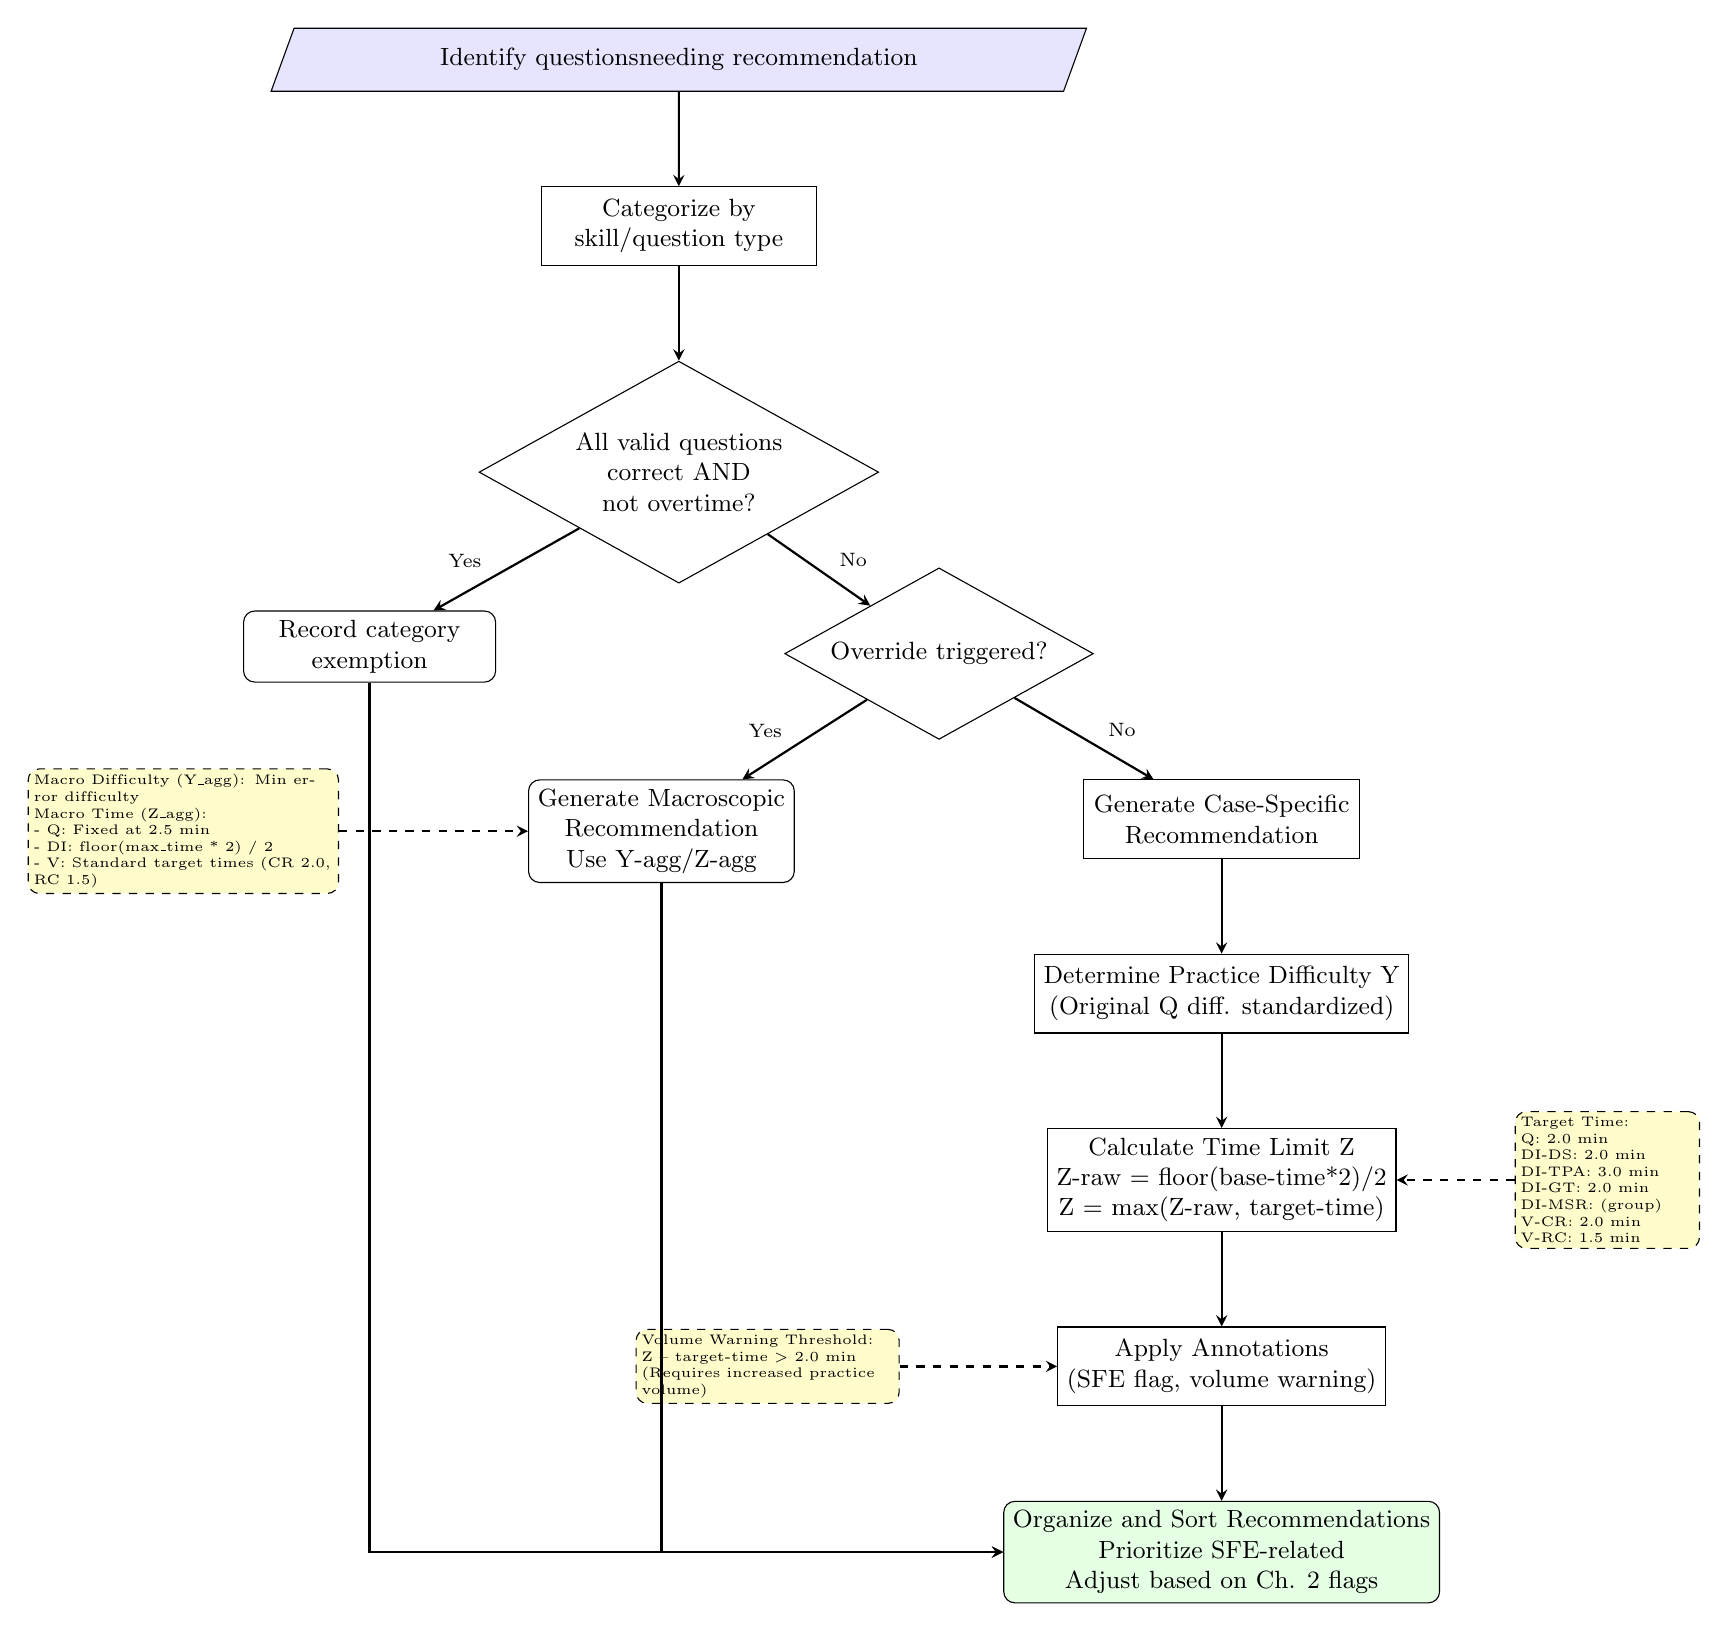
\begin{tikzpicture}[
    box/.style={rectangle, draw, rounded corners, minimum width=3.2cm, minimum height=0.9cm, text centered, font=\small, align=center},
    decision/.style={diamond, draw, aspect=1.8, minimum width=3.5cm, minimum height=1.2cm, text centered, font=\small, align=center},
    process/.style={rectangle, draw, minimum width=3.5cm, minimum height=1cm, text centered, font=\small, align=center},
    data/.style={trapezium, draw, trapezium left angle=70, trapezium right angle=110, minimum width=3cm, minimum height=0.8cm, text centered, font=\small},
    arrow/.style={->, >=stealth, thick},
    param/.style={rectangle, draw, dashed, rounded corners, fill=yellow!20, font=\tiny, inner sep=2pt},
    node distance=1.2cm
]
% Input Data
\node[data, fill=blue!10] (input) {Identify questions\\needing recommendation};

% Categorization
\node[process, below=of input] (categorize) {Categorize by\\skill/question type};

% Iterate through each category
\node[decision, below=of categorize] (exemption) {All valid questions\\correct AND\\not overtime?}; % <-- MODIFIED NODE TEXT

% Removed exemption_param node and its arrow

\node[box, below left=of exemption, xshift=-0.2cm, yshift=-0.2cm] (exempt) {Record category\\exemption}; % Adjusted position
\node[decision, below right=of exemption, xshift=0.2cm, yshift=-0.2cm] (override) {Override triggered?}; % Adjusted position

\node[box, below left=of override, xshift=0cm, yshift=-0.2cm] (macroscopic) {Generate Macroscopic\\Recommendation\\Use Y-agg/Z-agg}; % Adjusted position
\node[param, align=left,
      text width=3.8cm,   % 限定寬度以自動換行
      left=of macroscopic, xshift=-1.2cm]
  (macro_param) {
    Macro Difficulty (Y\_agg): Min error difficulty\\
    Macro Time (Z\_agg):\\
    - Q: Fixed at 2.5 min\\
    - DI: floor(max\_time * 2) / 2\\
    - V: Standard target times (CR 2.0, RC 1.5)
  };


% Generate Case-Specific Recommendation
\node[process, below right=of override, xshift=0cm, yshift=-0.2cm] (case_gen) {Generate Case-Specific\\Recommendation}; % Adjusted position

\node[process, below=of case_gen, yshift=0cm] (calc_y) {Determine Practice Difficulty Y\\(Original Q diff. standardized)};

\node[process, below=of calc_y] (calc_z) {Calculate Time Limit Z\\Z-raw = floor(base-time*2)/2\\Z = max(Z-raw, target-time)};
\node[param,
      right=of calc_z, xshift=0.3cm,
      align=left,           % 啟用多行左對齊
      text width=2.2cm]       % 自動斷行寬度
  (time_param) {
    Target Time:\\
    Q: 2.0 min\\
    DI-DS: 2.0 min\\
    DI-TPA: 3.0 min\\
    DI-GT: 2.0 min\\
    DI-MSR: (group)\\
    V-CR: 2.0 min\\
    V-RC: 1.5 min
  };


% 原先的 annotation 節點
\node[process, below=of calc_z,
      align=center]            % 啟用多行置中
  (annotation) {
    Apply Annotations\\
    (SFE flag, volume warning)
  };

% 調整 anno_param 節點,增加 align 與 text width
\node[param, left=of annotation, xshift=-0.8cm, 
      align=left,              % 啟用多行左對齊
      text width=3.2cm]          % 指定斷行寬度
  (anno_param) {
    Volume Warning Threshold:\\
    Z – target-time > 2.0 min\\
    (Requires increased practice volume)
  };

% Final Output
\node[box, below=of annotation, fill=green!10, yshift=0cm] (organize) {Organize and Sort Recommendations\\Prioritize SFE-related\\Adjust based on Ch. 2 flags};

% Arrow Connections
\draw[arrow] (input) -- (categorize);
\draw[arrow] (categorize) -- (exemption);
\draw[arrow] (exemption) -- node[above left, font=\scriptsize, pos=0.6] {Yes} (exempt);
\draw[arrow] (exemption) -- node[above right, font=\scriptsize, pos=0.6] {No} (override);
\draw[arrow] (override) -- node[above left, font=\scriptsize, pos=0.6] {Yes} (macroscopic);
\draw[arrow] (override) -- node[above right, font=\scriptsize, pos=0.6] {No} (case_gen);
\draw[arrow] (case_gen) -- (calc_y);
\draw[arrow] (calc_y) -- (calc_z);
\draw[arrow] (calc_z) -- (annotation);
\draw[arrow] (annotation) -- (organize);
\draw[arrow] (exempt) |- (organize);
\draw[arrow] (macroscopic) |- (organize);

% Removed arrow from exemption_param
% \draw[arrow, dashed] (exemption_param) -- (exemption); 
\draw[arrow, dashed] (macro_param) -- (macroscopic);
\draw[arrow, dashed] (time_param) -- (calc_z);
\draw[arrow, dashed] (anno_param) -- (annotation);
\end{tikzpicture}
}

\vspace{\baselineskip}
\caption{Flowchart for Chapter 7 Logic: Practice Recommendation Generation}
\label{fig:chapter7_logic}
\end{figure}
% ***** 圖表程式碼結束 *****

\textbf{Implementation Context:} This logic typically resides in the latter part of the main analysis function. Exemption checks require pre-calculating relevant metrics per category. Recommendation generation involves iterating through triggers or groups, applying conditional logic for exemption/override, calculating Y/Z using helper functions or inline logic based on section rules (aggregation, min/max), formatting text strings with annotations, and storing them (e.g., in a list of dictionaries). Focus rules are applied during the final organization phase. The flowchart in Figure \ref{fig:chapter7_logic} illustrates the core calculation steps for determining Y and Z for a single trigger point, which forms the basis for Q recommendations and is a pre-aggregation step for V/DI. To enhance the fluency and clarity of the generated report, AI-powered tools may optionally be utilized to assist in synthesizing the findings and recommendations into user-friendly prose.

\textbf{Rationale:} Provides a holistic, actionable summary translating complex quantitative diagnostics and parameterized recommendations into clear, user-friendly insights and next steps, maximizing the practical value of the analysis for the student.

\subsection{Chapter 8: Diagnostic Summary and Subsequent Actions}

\textbf{Objective:} Synthesize all analysis findings and recommendations into a comprehensive, easily understandable report for the student, \textbf{using exclusively natural language}.

\textbf{Report Structure and Content Synthesis:}
\begin{enumerate}
    \item \textbf{Opening Summary:} This initial section synthesizes key findings from Chapter 1, including: the assessed \texttt{time\_pressure} status (described naturally, e.g., "significant time pressure was likely experienced"), total time usage relative to the limit, and whether any data was deemed invalid due to end-section rushing (e.g., "analysis excludes X questions answered hastily at the end under pressure").
    \item \textbf{Performance Overview:} Summarizes Chapter 2 results descriptively: Relative performance across key dimensions (Q: 'Real' vs. 'Pure'; DI: 'Math Related' vs. 'Non-Math Related', types 'DS', 'TPA', etc.; V: Skill performance, 'CR' vs. 'RC') and difficulty levels (e.g., "Errors were concentrated in the High difficulty range," "Performance on 'Math Related' DI questions was significantly weaker than 'Non-Math Related'"). Mention reading time assessment for V if flagged.
    \item \textbf{Core Problem Diagnosis:} Translates Chapter 3 findings into narrative form: Describes primary error patterns identified (e.g., "A tendency towards calculation errors in Pure Quant questions was observed," "Difficulties in interpreting complex graph relationships under time pressure were noted in GT questions," "Logical flaws in evaluating assumptions were apparent in CR questions"). \textbf{Crucially highlights SFE findings} using descriptive language (e.g., "Particular attention is needed for errors occurring on questions below your typical mastery level in [Skill/Type], suggesting instability in applying fundamental concepts."). Includes MSR-specific time issues for DI if detected.
    \item \textbf{Pattern Observation:} Integrates Chapter 5 alerts: Notes risks associated with early-stage rapid responses or potential carelessness if the \texttt{carelessness\_issue} flag was triggered (e.g., "A pattern of rapid, incorrect answers suggests that focusing on accuracy over speed may be beneficial").
    \item \textbf{Foundational Consolidation Advisory:} Explicitly states which skills/types require systematic foundational work based on Chapter 6 override triggers (e.g., "Systematic review and practice of the fundamentals for [Skill/Type] is recommended due to overall performance patterns").
    \item \textbf{Practice Plan Presentation:} Presents the full, organized list of recommendations generated in Chapter 7, ensuring clarity and including all annotations (priority, volume alerts, focus rules, exemptions) in natural language descriptions within the recommendation text itself.
    \item \textbf{Guidance for Subsequent Actions:} Provides actionable next steps:
    \begin{itemize}
        \item \textbf{Guiding Reflection Questions:} Poses targeted, open-ended questions based on the specific diagnoses to prompt student self-assessment (incorporating MSR-specific questions for DI).
        \item \textbf{Secondary Evidence Review Suggestion:} Explains \textit{when} (e.g., uncertain recall, need pattern confirmation) and \textit{how} (e.g., review recent logs, focus on specific error types) to use past practice data.
        \item \textbf{Qualitative Analysis Suggestion:} Explains \textit{when} (e.g., root cause remains unclear after other steps) and \textit{how} (e.g., provide detailed walkthroughs for specific problem types) to engage in deeper analysis, potentially with an advisor.
    \end{itemize}
\end{enumerate}

\textbf{Core Constraint Adherence:} The implementation generating this chapter\'s output must rigorously avoid exposing internal variable names (e.g., \texttt{time\_pressure}, \texttt{is\_invalid}, \texttt{special\_focus\_error}), specific performance flags, numerical thresholds, or calculation details. All findings must be translated into clear, easily understandable, descriptive prose suitable for the end-user (student).

\textbf{Implementation Context:} This is typically handled by a dedicated \texttt{generate\_report\_*} function that receives all computed metrics, flags, lists, and generated recommendation texts as arguments. It uses conditional statements (\texttt{if/else}) and formatted strings (\texttt{f-strings}) to assemble the report sections based on the presence and values of these inputs, ensuring adherence to the natural language constraint.

\textbf{Rationale:} Provides a holistic, actionable summary translating complex quantitative diagnostics and parameterized recommendations into clear, user-friendly insights and next steps, maximizing the practical value of the analysis for the student.

\subsection{Illustrative Example: Simplified Question Journey}

To illustrate how the framework processes a single question, consider this simplified hypothetical example for a Quant ('Pure') question:

\textbf{Input Data:}
\begin{itemize}
    \item \texttt{question\_id}: Q5
    \item \texttt{question\_time}: 3.2 min
    \item \texttt{is\_correct}: False
    \item \texttt{question\_difficulty}: 650
    \item \texttt{question\_position}: 10 (out of 21)
    \item \texttt{question\_type}: 'Pure'
    \item \texttt{question\_fundamental\_skill}: 'Algebra'
    \item (Assume \texttt{total\_test\_time} = 43 min, \texttt{max\_allowed\_time} = 45 min, implies \texttt{time\_pressure} = False based on Q/DI rule)
    \item (Assume \texttt{average\_time\_per\_type} for 'Pure' = 2.1 min)
    \item (Assume \texttt{max\_mastered\_difficulty} for 'Algebra' = 700)
\end{itemize}

\textbf{Framework Steps Applied:}
\begin{enumerate}
    \item \textbf{Chapter 1 (Validity/Overtime):} 
        \begin{itemize}
            \item \texttt{time\_pressure} is False. 
            \item \texttt{question\_position} is not in the last third, and \texttt{question\_time} > 1.0 min $\rightarrow$ \texttt{is\_invalid} = False. (Data is valid).
            \item The \texttt{overtime\_threshold} for Q (no pressure) is 3.0 min. Since 3.2 min > 3.0 min $\rightarrow$ \texttt{overtime} = True.
        \end{itemize}
    \item \textbf{Chapter 2 (Performance - Context):} This question contributes to the overall metrics for 'Pure' type, 'Algebra' skill, and the corresponding difficulty band (e.g., "Medium / 605+").
    \item \textbf{Chapter 3 (Root Cause):}
        \begin{itemize}
            \item Time Classification: 3.2 min is not < (2.1 * 0.75) $\rightarrow$ \texttt{is\_relatively\_fast} = False. Since \texttt{overtime} is True $\rightarrow$ \texttt{is\_slow} = True.
            \item SFE Check: \texttt{is\_correct} is False, and \texttt{question\_difficulty} (650) < \texttt{max\_mastered\_difficulty} (700) $\rightarrow$ \texttt{special\_focus\_error} = True.
            \item Scenario: Slow \& Wrong \& SFE.
        \end{itemize}
    \item \textbf{Chapter 6 (Coverage - Check):} Check if 'Algebra' skill has \texttt{error\_rate} or \texttt{overtime\_rate} > 50\%. (Assume for this example it does not $\rightarrow$ \texttt{skill\_override\_triggered}['Algebra'] = False).
    \item \textbf{Chapter 7 (Recommendation):}
        \begin{enumerate}
            \item Trigger: Incorrect question (Q5).
            \item Exemption/Override: Not exempt (based on other Algebra questions) and not overridden.
            \item Y (Difficulty): Map 650 to label (e.g., "Medium / 605+").
            \item Z (Time): \texttt{is\_slow} is True. \texttt{base\_time} = 3.2 - 0.5 = 2.7. \texttt{Z\_raw} = floor(2.7 * 2) / 2 = floor(5.4) / 2 = 5.0 / 2 = 2.5. \texttt{target\_time} for Q is 2.0. \texttt{Z} = max(2.5, 2.0) = 2.5 min.
            \item Annotation: Prepend "*Fundamental mastery potentially unstable:* Practice Algebra ('Pure') problems at Medium / 605+ difficulty, starting with a 2.5 min time limit (target 2.0 min)."
        \end{enumerate}
\end{enumerate}
This example shows the flow from raw data through flagging (overtime, SFE) to a specific, annotated recommendation based on the framework's rules.

\subsection{Implementation Details}

The unified diagnostic framework described herein has been implemented as a set of Python scripts (\texttt{gmat\_q\_analyzer.py}, \texttt{gmat\_di\_analyzer.py}, \texttt{gmat\_v\_analyzer.py}), one for each GMAT section. The development followed an iterative process involving requirements analysis based on the methodological documents (\texttt{en-gmat-\*.md}), coding, testing with sample datasets (\texttt{testset-\*.csv}), debugging, and refinement based on analysis outcomes and evolving reporting requirements.

\textbf{Core Technologies:}
\begin{itemize}
    \item \textbf{Python:} The primary programming language.
    \item \textbf{Pandas:} Extensively used for data manipulation, including reading CSV files, data cleaning (handling missing values, type conversion), filtering, grouping, aggregation, and time-series operations where applicable. DataFrame structures are central to storing and processing the per-question data and analytical results.
    \item \textbf{NumPy:} Utilized for numerical operations, handling potential \texttt{NaN} values, and creating placeholder data structures (e.g., spacer rows using \texttt{np.nan}).
    \item \textbf{Argparse:} Employed for command-line argument parsing, allowing users to specify input/output file paths and optional flags (e.g., overriding \texttt{time\_pressure} status).
\end{itemize}

\textbf{Development Challenges \& Solutions:}
\begin{itemize}
    \item \textbf{Environment \& Dependencies:} Initial challenges included resolving Python interpreter path issues and managing dependencies (\texttt{pandas}, \texttt{numpy}). The use of Python virtual environments (\texttt{venv}) was adopted to ensure consistent and isolated execution environments, addressing \texttt{externally-managed-environment} errors related to PEP 668.
    \item \textbf{Data Inconsistencies:} Handling variations in input CSV formats, such as extra commas in headers or differing column names (e.g., \texttt{V\_b}, \texttt{DI\_b} vs. a consistent \texttt{question\_difficulty}), required robust parsing logic (e.g., using \texttt{usecols} in \texttt{pd.read\_csv}, dynamic column renaming). Encoding issues were addressed by attempting multiple common encodings (\texttt{utf-8}, \texttt{gbk}, \texttt{cp950}).
    \item \textbf{Logic Implementation:} Translating the sometimes complex, multi-conditional logic from the markdown documents into precise code required careful structuring, particularly for overtime calculations, SFE detection, and recommendation generation involving multiple interacting rules (override, exemption, focus). Helper functions were created to encapsulate reusable logic (e.g., difficulty mapping, safe division, Z-time calculation, MSR/RC group processing).
    \item \textbf{Pandas Operations:} Specific \texttt{pandas} operations occasionally led to errors (e.g., ambiguity in boolean operations on DataFrames, errors during DataFrame initialization with specific structures like \texttt{[[]] * n}), necessitating refactoring to use element-wise operations or more robust initialization methods (\texttt{pd.DataFrame(np.nan, ...)}).
    \item \textbf{Evolving Requirements:} The most significant evolution was the increasing demand for report granularity. Initial implementations produced summary-level reports, but later iterations required significant refactoring to generate detailed, per-question diagnostics, actions, reflections, and evidence prompts, necessitating the creation of \texttt{get\_detailed\_diagnosis\_*} functions and modifications to the main analysis loop and report generation logic across all three scripts.
    \item \textbf{Debugging:} Identifying the root cause of errors often involved tracing data flow through the DataFrame, checking intermediate values, and verifying that conditional logic correctly handled edge cases (e.g., division by zero, empty data subsets after filtering). \texttt{NameError} and \texttt{KeyError} issues were common during refactoring, requiring careful checking of variable scope and dictionary key handling.
\end{itemize}

\textbf{Output Data Format (Annotated CSV):}
In addition to the natural language summary report, the Python scripts generate an output CSV file (e.g., \texttt{testset-q-analyzed.csv}). This file contains all the original input data plus several new columns representing the diagnostic flags calculated during the analysis. Key added columns include:

\begin{itemize}
    \item \texttt{difficulty\_label}: The standardized difficulty category (e.g., "Medium / 605+").
    \item \texttt{time\_pressure}: Boolean flag indicating if overall time pressure was detected (Chapter 1).
    \item \texttt{is\_invalid}: Boolean flag indicating if the question data was excluded due to extreme rushing under time pressure (Chapter 1).
    \item \texttt{overtime} (or variants like \texttt{group\_overtime}): Boolean flag indicating if the question (or group) exceeded the calculated overtime threshold based on the *filtered* data (Chapter 1).
    \item \texttt{is\_relatively\_fast}: Boolean flag indicating if the question was answered significantly faster than the average for its type (Chapter 3).
    \item \texttt{is\_slow}: Boolean flag, essentially mirroring the \texttt{overtime} flag for consistency in time classification (Chapter 3).
    \item \texttt{max\_mastered\_difficulty}: The highest difficulty level mastered within the relevant skill/type category based on correct answers (Chapter 3).
    \item \texttt{special\_focus\_error}: A Boolean indicator signifying an error made on a question possessing a difficulty level inferior to the user's attained \texttt{max\_mastered\_difficulty} within that specific subject category (as specified in Chapter 3).
    \item \texttt{skill\_override\_triggered} / \texttt{override\_triggered}: Boolean flag indicating if a coverage rule was triggered for the question's skill/type (Chapter 6).
    \item \texttt{Recommendation\_Y}: The suggested practice difficulty level (String label).
    \item \texttt{Recommendation\_Z}: The suggested starting practice time limit (Numeric, minutes).
    \item \texttt{Diagnostic\_Notes}: Text field containing generated diagnostic comments or recommendation details.
\end{itemize}
This annotated CSV allows for detailed review and further analysis of the framework's per-question conclusions.

\textbf{Current State:} The resulting Python scripts represent functional implementations of the diagnostic framework. They successfully ingest section-specific GMAT data, apply the complex analytical logic outlined in Chapters 0-7, handle various data edge cases, and produce detailed output CSV files containing both per-question diagnostic flags and a comprehensive, natural-language summary report adhering to the structure of Chapter 8. The scripts are designed to be run from the command line, providing a practical tool for automated GMAT performance analysis.

\section{Conclusion}

The primary value of this framework, as detailed in this technical report, lies in its systematic and unified approach to formalizing the complex process of GMAT performance diagnosis across multiple sections. It provides a transparent, structured, and potentially automatable methodology moving beyond simple metrics. 

As documentation focused on the framework's design, readers should note its current limitations. The specific parameter values used in the implementation represent informed heuristics derived from initial analysis and expert consultation, rather than statistically optimized values derived from large-scale empirical validation. While preliminary comparisons to expert analysis are encouraging, rigorous validation of the framework's diagnostic accuracy and effectiveness remains a crucial next step for future development.

The unified GMAT diagnostic framework presented offers a systematic, multi-faceted approach to analyzing student performance across the Quantitative, Data Insights, and Verbal sections. By adhering to a consistent chapter-based structure while accommodating section-specific nuances through parameterized logic and tailored analyses, the framework moves beyond superficial score reporting to identify root causes of errors and inefficiencies. Key strengths include:

\begin{itemize}
    \item \textbf{Comprehensive Scope:} Addresses time management, data validity, accuracy, efficiency, behavioral patterns, and foundational knowledge across all scored sections.
    \item \textbf{Depth of Analysis:} Employs concepts like relative time performance, \texttt{special\_focus\_error} detection, and coverage rules to provide nuanced diagnoses based on operationalized parameters.
    \item \textbf{Actionable Output:} Generates personalized practice plans with specific difficulty (\texttt{Y}/\texttt{Y\_agg}) and time (\texttt{Z}/\texttt{Z\_agg}) parameters, alongside structured guidance for self-reflection and further analysis.
    \item \textbf{Standardization \& Adaptability:} Provides a consistent analytical process applicable to Q, DI, and V, ensuring comparable insights while respecting the unique demands of each section, as evidenced by the successful implementation across three distinct Python modules.
\end{itemize}

This framework, validated through empirical testing and refinement, empowers students and instructors with detailed, data-driven insights, facilitating more targeted preparation and ultimately aiming for improved GMAT performance.

\section{Future Directions}

Building upon the established framework and its current implementation, several avenues for future development and application are envisioned:

\begin{enumerate}
    \item \textbf{Web-Based Implementation:} To enhance accessibility and utility, the diagnostic framework is planned for implementation as an automated, user-facing tool integrated into a web platform. This would allow students to upload their score data (e.g., via CSV or potentially through direct API integration if available) and receive instant, standardized diagnostic reports through a user-friendly interface.
   \item \textbf{Rigorous Parameter Optimization and Validation:} Beyond initial heuristics, future work involves rigorously validating and optimizing framework parameters (e.g., time thresholds, speed factors, SFE sensitivity, coverage rules) and predictive accuracy. Hyperparameter optimization methods like Grid Search will be used on larger student datasets to find parameter sets maximizing concordance between the framework's diagnoses and validated metrics or expert assessments, enhancing diagnostic and predictive effectiveness.
    \item \textbf{Integration of Qualitative Feedback:} Explore methods to integrate qualitative student feedback (e.g., self-reported reasons for errors, confidence levels) directly into the diagnostic process, potentially refining the root cause analysis beyond purely quantitative data.
    \item \textbf{Longitudinal Analysis:} Extend the framework to analyze performance trends over multiple test administrations or practice sessions for a single student, identifying patterns of improvement or persistent weaknesses.
\end{enumerate}

\newpage % Start Appendix on a new page
    \appendix
    \section*{Appendix A: Diagnostic Parameter Tags and Descriptions}
    
    This appendix lists the standardized diagnostic parameter tags used by the framework across the Q, DI, and V sections, along with their English descriptions. These parameters represent potential root causes for errors or inefficiencies identified during the analysis.
    
    \vspace{1em}
    \begin{tabular}{|l|p{9cm}|}
    \hline
    \textbf{Parameter Tag} & \textbf{English Description} \\
    \hline
    \multicolumn{2}{|c|}{\textbf{Reading / Comprehension / Interpretation}} \\
    \hline
    \texttt{Q\_READING\_COMPREHENSION\_ERROR} & Q Reading: Difficulty understanding word problem text (Real Context) \\
    \texttt{Q\_PROBLEM\_UNDERSTANDING\_ERROR} & Q Problem Understanding: Misinterpretation of question requirements/logic \\
    \texttt{DI\_READING\_COMPREHENSION\_ERROR} & DI Reading Comprehension: Error/Difficulty understanding text (Math/Non-Math) \\
    \texttt{DI\_GRAPH\_TABLE\_INTERPRETATION\_ERROR} & DI Graph/Table Interpretation: Error/Difficulty interpreting visual data \\
    \texttt{CR\_READING\_BASIC\_OMISSION} & CR Reading: Basic comprehension omission \\
    \texttt{CR\_READING\_DIFFICULTY\_STEM} & CR Reading: Stem comprehension difficulty (keyword/syntax/logic/domain) \\
    \texttt{CR\_QUESTION\_UNDERSTANDING\_MISINTERPRETATION} & CR Question Understanding: Misinterpretation of question task \\
    \texttt{RC\_READING\_VOCAB\_BOTTLENECK} & RC Reading: Vocabulary bottleneck \\
    \texttt{RC\_READING\_SENTENCE\_STRUCTURE\_DIFFICULTY} & RC Reading: Difficulty parsing complex sentence structures \\
    \texttt{RC\_READING\_PASSAGE\_STRUCTURE\_DIFFICULTY} & RC Reading: Difficulty grasping passage structure \\
    \texttt{RC\_READING\_DOMAIN\_KNOWLEDGE\_GAP} & RC Reading: Lack of background knowledge in specific domain \\
    \texttt{RC\_QUESTION\_UNDERSTANDING\_MISINTERPRETATION} & RC Question Understanding: Misinterpretation of question focus \\
    \hline
    \multicolumn{2}{|c|}{\textbf{Concept / Logic Application}} \\
    \hline
    \texttt{Q\_CONCEPT\_APPLICATION\_ERROR} & Q Concept Application: Error applying mathematical concepts/formulas \\
    \texttt{DI\_CONCEPT\_APPLICATION\_ERROR} & DI Concept Application (Math): Error applying mathematical concepts/formulas \\
    \texttt{DI\_LOGICAL\_REASONING\_ERROR} & DI Logical Reasoning (Non-Math): Error in inherent logical reasoning/judgment \\
    \texttt{CR\_REASONING\_CHAIN\_ERROR} & CR Reasoning: Error in analyzing logical chain (premise/conclusion/relation) \\
    \texttt{CR\_REASONING\_ABSTRACTION\_DIFFICULTY} & CR Reasoning: Difficulty with abstract logic/terminology \\
    \texttt{CR\_REASONING\_PREDICTION\_ERROR} & CR Reasoning: Incorrect or missing prediction \\
    \texttt{CR\_REASONING\_CORE\_ISSUE\_ID\_DIFFICULTY} & CR Reasoning: Difficulty identifying the core issue \\
    \texttt{RC\_REASONING\_INFERENCE\_WEAKNESS} & RC Reasoning: Weak inference skills (prediction/detail/tone) \\
    \hline
    \multicolumn{2}{|c|}{\textbf{Data Handling / Calculation / Location}} \\
    \hline
    \texttt{Q\_CALCULATION\_ERROR} & Q Calculation: Error in mathematical computation \\
    \texttt{DI\_DATA\_EXTRACTION\_ERROR} & DI Data Extraction (GT): Error extracting data from graphs/tables \\
    \texttt{DI\_INFORMATION\_EXTRACTION\_INFERENCE\_ERROR} & DI Info Extraction/Inference (GT/MSR Non-Math): Error locating/inferring info \\
    \texttt{DI\_CALCULATION\_ERROR} & DI Calculation: Error in mathematical computation \\
    \texttt{RC\_READING\_INFO\_LOCATION\_ERROR} & RC Reading: Error locating/understanding key information \\
    \texttt{RC\_READING\_KEYWORD\_LOGIC\_OMISSION} & RC Reading: Omission of keywords/logic \\
    \texttt{RC\_LOCATION\_ERROR\_INEFFICIENCY} & RC Location: Incorrect or inefficient information location \\
    \hline
    \multicolumn{2}{|c|}{\textbf{Section/Type Specific (MSR / CR / RC)}} \\
    \hline
    \texttt{DI\_MULTI\_SOURCE\_INTEGRATION\_ERROR} & DI Multi-Source Integration (MSR): Error integrating info across sources \\
    \texttt{DI\_MSR\_READING\_COMPREHENSION\_BARRIER} & DI MSR Reading Barrier: Excessive overall reading time for the group \\
    \texttt{DI\_QUESTION\_TYPE\_SPECIFIC\_ERROR} & DI Question Type Specific Error (e.g., MSR Non-Math sub-type) \\
    \texttt{CR\_AC\_ANALYSIS\_UNDERSTANDING\_DIFFICULTY} & CR AC Analysis: Difficulty understanding the answer choice itself \\
    \texttt{CR\_AC\_ANALYSIS\_RELEVANCE\_ERROR} & CR AC Analysis: Error judging answer choice relevance \\
    \texttt{CR\_AC\_ANALYSIS\_DISTRACTOR\_CONFUSION} & CR AC Analysis: Confusion with strong distractors \\
    \texttt{CR\_METHOD\_PROCESS\_DEVIATION} & CR Method: Deviation from standard procedure \\
    \texttt{CR\_METHOD\_TYPE\_SPECIFIC\_ERROR} & CR Method: Error/unfamiliarity with specific question type method (Specify type) \\
    \texttt{RC\_READING\_PRECISION\_INSUFFICIENT} & RC Reading: Insufficient precision (close reading/location issue) \\
    \texttt{RC\_METHOD\_INEFFICIENT\_READING} & RC Method: Inefficient reading method (e.g., over-reading) \\
    \texttt{RC\_AC\_ANALYSIS\_DIFFICULTY} & RC AC Analysis: Difficulty understanding/discriminating choices (meaning/mapping) \\
    \hline
    \multicolumn{2}{|c|}{\textbf{Foundational Mastery}} \\
    \hline
    \texttt{Q\_FOUNDATIONAL\_MASTERY\_INSTABILITY\_SFE} & Q Foundational Mastery: Unstable application (Special Focus Error) \\
    \texttt{DI\_FOUNDATIONAL\_MASTERY\_INSTABILITY\_SFE} & DI Foundational Mastery: Unstable application (Special Focus Error) \\
    \texttt{FOUNDATIONAL\_MASTERY\_INSTABILITY\_SFE} & V Foundational Mastery: Unstable application (Special Focus Error) \\
    \hline
    \multicolumn{2}{|c|}{\textbf{Efficiency Bottlenecks}} \\
    \hline
    \texttt{Q\_EFFICIENCY\_BOTTLENECK\_READING} & Q Efficiency Bottleneck: Reading time (Real Context) \\
    \texttt{Q\_EFFICIENCY\_BOTTLENECK\_CONCEPT} & Q Efficiency Bottleneck: Concept recall/application time \\
    \texttt{Q\_EFFICIENCY\_BOTTLENECK\_CALCULATION} & Q Efficiency Bottleneck: Calculation time \\
    \texttt{DI\_EFFICIENCY\_BOTTLENECK\_READING} & DI Efficiency Bottleneck: Reading/Comprehension time (Math/Non-Math) \\
    \texttt{DI\_EFFICIENCY\_BOTTLENECK\_CONCEPT} & DI Efficiency Bottleneck: Concept/Formula application time (Math) \\
    \texttt{DI\_EFFICIENCY\_BOTTLENECK\_CALCULATION} & DI Efficiency Bottleneck: Calculation time \\
    \texttt{DI\_EFFICIENCY\_BOTTLENECK\_LOGIC} & DI Efficiency Bottleneck: Logical reasoning time (Non-Math) \\
    \texttt{DI\_EFFICIENCY\_BOTTLENECK\_GRAPH\_TABLE} & DI Efficiency Bottleneck: Graph/Table interpretation time \\
    \texttt{DI\_EFFICIENCY\_BOTTLENECK\_INTEGRATION} & DI Efficiency Bottleneck: Multi-source integration time (MSR) \\
    \texttt{CR\_READING\_TIME\_EXCESSIVE} & CR Reading: Excessive time spent reading \\
    \texttt{CR\_REASONING\_TIME\_EXCESSIVE} & CR Reasoning: Excessive time spent on logical thinking \\
    \texttt{CR\_AC\_ANALYSIS\_TIME\_EXCESSIVE} & CR AC Analysis: Excessive time spent eliminating choices \\
    \texttt{RC\_READING\_SPEED\_SLOW\_FOUNDATIONAL} & RC Reading: Slow reading speed (foundational issue) \\
    \texttt{RC\_LOCATION\_TIME\_EXCESSIVE} & RC Location: Excessive time spent locating information (re-locating) \\
    \texttt{RC\_REASONING\_TIME\_EXCESSIVE} & RC Reasoning: Excessive time spent on deep thinking \\
    \texttt{RC\_AC\_ANALYSIS\_TIME\_EXCESSIVE} & RC AC Analysis: Excessive time spent eliminating choices \\
    \texttt{EFFICIENCY\_BOTTLENECK\_[AREA]} & Generic V Efficiency Issue: Bottleneck in [Specific Area] (Specify Area: READING, REASONING, LOCATION, AC\_ANALYSIS) \\
    \hline
    \multicolumn{2}{|c|}{\textbf{Behavioral Patterns}} \\
    \hline
    \texttt{Q\_CARELESSNESS\_DETAIL\_OMISSION} & Q Behavior: Carelessness - Detail omission/misread (Implied in Fast \\& Wrong) \\\\
    \texttt{DI\_CARELESSNESS\_DETAIL\_OMISSION} & DI Behavior: Carelessness - Detail omission/misread (Implied in Fast \\& Wrong) \\\\
    \texttt{BEHAVIOR\_CARELESSNESS\_ISSUE} & Behavior Pattern: Carelessness issue (overall high fast-wrong rate > 25\%) \\\\
    \texttt{BEHAVIOR\_EARLY\_RUSHING\_FLAG\_RISK} & Behavior Pattern: Rushing early in section (< 1.0 min, Note flag for review risk) \\\\
    \texttt{BEHAVIOR\_GUESSING\_HASTY} & Behavior Pattern: Hasty response suggesting guessing/rushing \\\\
    \hline
    \end{tabular}
    
    \end{document}